\resizebox{0.97\textwidth}{!}{%
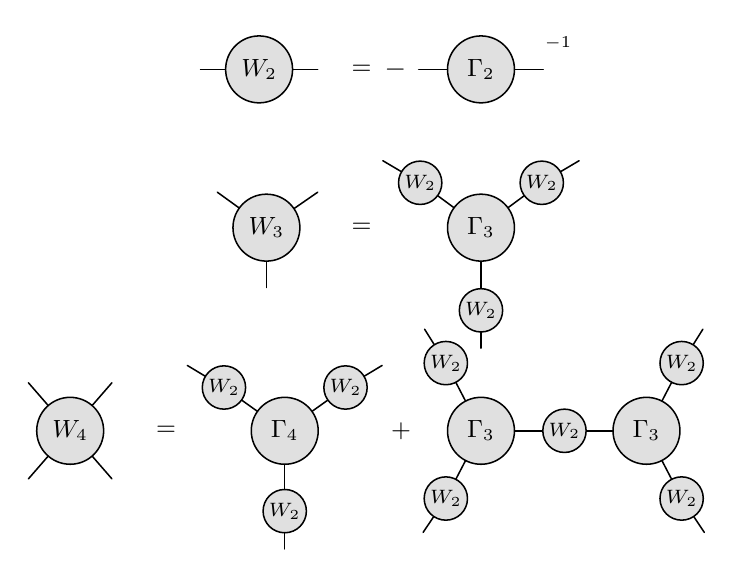
\begin{tikzpicture}[x=0.93cm,y=1cm,xshift=0.28cm,baseline=(current bounding box.center),
  line cap=round,line join=round,
  every node/.style={font=\small},
  L/.style={line width=.55pt},
  v/.style={draw,line width=.55pt,circle,fill=black!12,minimum size=8.5mm,inner sep=0pt},
  e/.style={draw,line width=.55pt,circle,fill=black!12,minimum size=5.5mm,inner sep=0pt}]

  %% ---- row 1:  --(W_2)--  =  - --(Gamma_2)--^{-1}
  \draw[L] (1.78,4.59) -- (3.38,4.59);
  \draw[L] (4.76,4.59) -- (6.46,4.59);

  %% ---- row 2:  W_3  =  Gamma_3 dressed by three W_2 on its legs
  % W_3 legs
  \draw[L] (2.68,2.58) -- (2.01,3.03);
  \draw[L] (2.68,2.58) -- (3.38,3.03);
  \draw[L] (2.68,2.58) -- (2.68,1.82);
  % Gamma_3 legs, each carrying a W_2 which continues to an external stub
  \draw[L] (5.61,2.58) -- (4.78,3.15) -- (4.27,3.43);
  \draw[L] (5.61,2.58) -- (6.44,3.15) -- (6.95,3.43);
  \draw[L] (5.61,2.58) -- (5.61,1.53) -- (5.61,1.05);

  %% ---- row 3:  W_4  =  Gamma_4 term  +  Gamma_3--W_2--Gamma_3 term
  % W_4 legs
  \draw[L] (0,0) -- (-0.57,0.61);
  \draw[L] (0,0) -- (0.57,0.61);
  \draw[L] (0,0) -- (-0.57,-0.61);
  \draw[L] (0,0) -- (0.57,-0.61);
  % Gamma_4 term (drawn in the source with three dressed legs)
  \draw[L] (2.93,0) -- (2.10,0.55) -- (1.60,0.83);
  \draw[L] (2.93,0) -- (3.76,0.55) -- (4.26,0.83);
  \draw[L] (2.93,0) -- (2.93,-1.02) -- (2.93,-1.50);
  % Gamma_3 -- W_2 -- Gamma_3 term
  \draw[L] (5.61,0) -- (7.87,0);
  \draw[L] (5.61,0) -- (5.13,0.86) -- (4.84,1.29);
  \draw[L] (5.61,0) -- (5.13,-0.86) -- (4.82,-1.29);
  \draw[L] (7.87,0) -- (8.35,0.86) -- (8.64,1.29);
  \draw[L] (7.87,0) -- (8.35,-0.86) -- (8.66,-1.29);

  %% ---- blobs (drawn last so they mask the leg stubs underneath)
  % row 1
  \node[v] at (2.58,4.59) {$W_2$};
  \node    at (3.98,4.59) {$=$};
  \node[font=\normalsize] at (4.44,4.59) {$-$};
  \node[v] at (5.61,4.59) {$\Gamma_2$};
  \node    at (6.66,4.92) {$\scriptstyle -1$};
  % row 2
  \node[v] at (2.68,2.58) {$W_3$};
  \node    at (3.98,2.58) {$=$};
  \node[v] at (5.61,2.58) {$\Gamma_3$};
  \node[e] at (4.78,3.15) {\scriptsize$W_2$};
  \node[e] at (6.44,3.15) {\scriptsize$W_2$};
  \node[e] at (5.61,1.53) {\scriptsize$W_2$};
  % row 3
  \node[v] at (0,0) {$W_4$};
  \node    at (1.31,0) {$=$};
  \node[v] at (2.93,0) {$\Gamma_4$};
  \node[e] at (2.10,0.55) {\scriptsize$W_2$};
  \node[e] at (3.76,0.55) {\scriptsize$W_2$};
  \node[e] at (2.93,-1.02) {\scriptsize$W_2$};
  \node    at (4.52,0) {$+$};
  \node[v] at (5.61,0) {$\Gamma_3$};
  \node[e] at (6.75,0) {\scriptsize$W_2$};
  \node[v] at (7.87,0) {$\Gamma_3$};
  \node[e] at (5.13,0.86) {\scriptsize$W_2$};
  \node[e] at (5.13,-0.86) {\scriptsize$W_2$};
  \node[e] at (8.35,0.86) {\scriptsize$W_2$};
  \node[e] at (8.35,-0.86) {\scriptsize$W_2$};
\end{tikzpicture}%
}
